\chapter{Results}
\label{chap:results}
\lhead{\emph{Results}}

\section{Introduction}

The results of this study are presented in this section.

\section{First Sprint - Global Generic}
\section{Second Sprint - Global Generic Analysis Resized}

\newpage

\section{Analysis Tesseract Separate Folders}


\begin{figure}[ht]
    \centering
    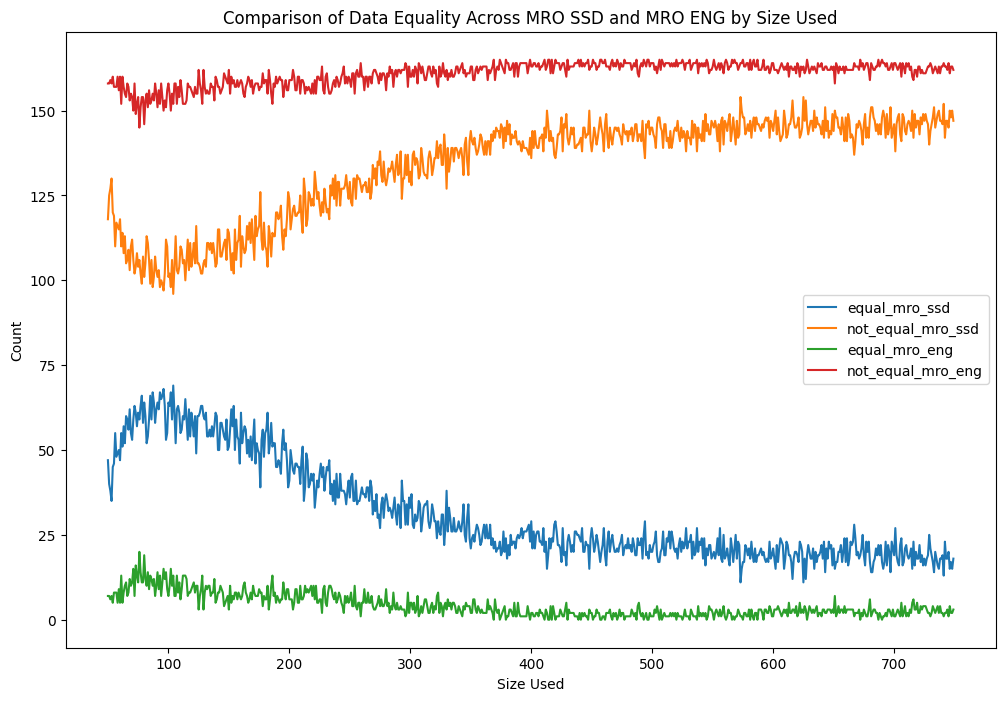
\includegraphics[width=0.9\textwidth]{Figures/Results/sipa_02/count_analysis.png}
    \caption[Count Analysis]{Sipa 2 Count Analysis}
    \label{fig:Sipa 2 Count Analysis}
\end{figure}

The chart presented primarily emphasizes the blue line, which signifies the count of Masked Red OTSU. This line is of particular importance. At size 100, we observe the peak read count.

This establishes the dimensions to which the images will be resized for each of the subsequent directories.


\newpage

\subsubsection{Sipa 2 Contrast Analysis on MRO SSD}

\begin{figure}[ht]
    \centering
    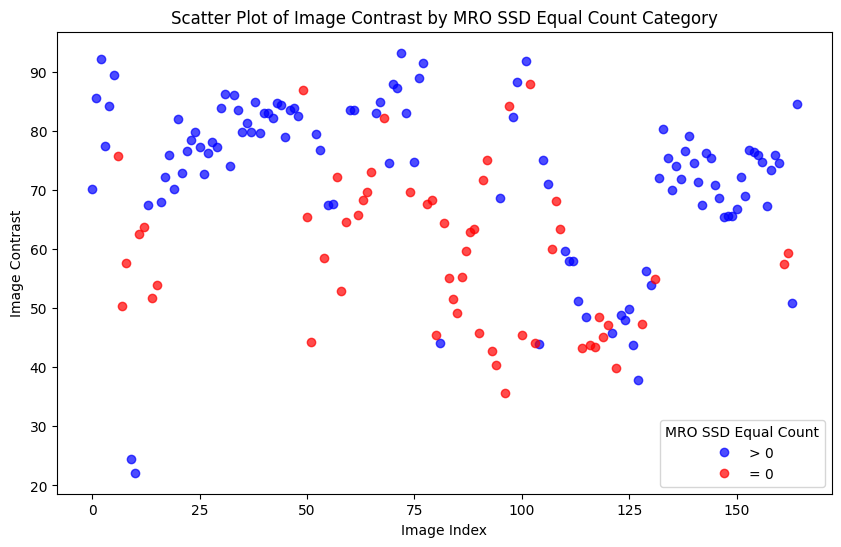
\includegraphics[width=0.9\textwidth]{Figures/Results/sipa_02/contrast.png}
    \caption[Sipa 2 Contrast Analysis on MRO SSD]{Sipa 2 Contrast Analysis on MRO SSD}
    \label{fig:Sipa 2 Contrast Analysis on MRO SSD}
\end{figure}

The scatter plot of image contrast shows that there is a wide range of contrast levels for both categories of images (MRO SSD EQUAL COUNT greater than 0 and equal to 0). This means that the contrast of images in both categories is highly variable. Additionally, there is significant overlap in the contrast values of both categories, suggesting that the contrast of an image may not be a strong indicator of whether the MRO SSD EQUAL COUNT is greater than 0 or not.

There are a few outliers in the MRO SSD EQUAL COUNT greater than 0 category with particularly high contrast levels. However, these outliers do not significantly change the overall pattern of the scatter plot.

In summary, the scatter plot of image contrast does not provide any clear evidence that the contrast of an image is a good predictor of the MRO SSD EQUAL COUNT value.

\newpage

\subsubsection{Sipa 2 Brightness Analysis on MRO SSD}


\begin{figure}[ht]
    \centering
    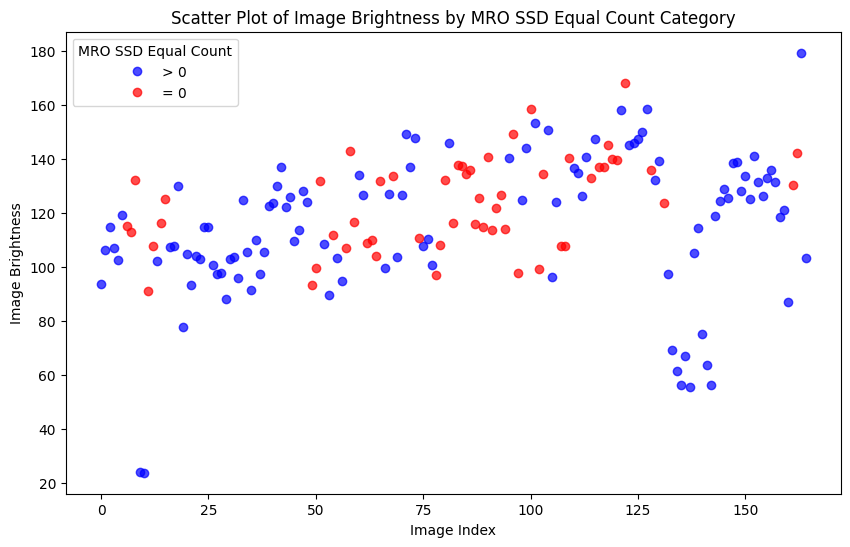
\includegraphics[width=0.9\textwidth]{Figures/Results/sipa_02/brightness.png}
    \caption[Sipa 2 Brightness Analysis on MRO SSD]{Sipa 2 Brightness Analysis on MRO SSD}
    \label{fig:Sipa 2 Brightness Analysis on MRO SSD}
\end{figure}



The scatter plot of image brightness shows that both categories of images (MRO SSD EQUAL COUNT greater than 0 and equal to 0) have a wide range of brightness values. This means that the brightness of images in both categories is highly variable. Additionally, there is no clear pattern or correlation between the MRO SSD EQUAL COUNT category and the brightness of the images. This suggests that the brightness of an image may not be a good predictor of whether the MRO SSD EQUAL COUNT is greater than 0 or not.

There are a few outliers in the MRO SSD EQUAL COUNT greater than 0 category with particularly high brightness levels. However, these outliers do not significantly change the overall pattern of the scatter plot.

In summary, the scatter plot of image brightness does not provide any clear evidence that the brightness of an image is a good predictor of the MRO SSD EQUAL COUNT value.

\newpage

% TODO: Add SD Analysis

\subsection{Sipa 2}
\subsection{Sipa 3}
\subsection{Sipa 4}
\subsection{Sipa 5}
\subsection{Sipa 6}
\subsection{Sipa 7}
\subsection{Sipa 8}
\subsection{Sipa 9}
\subsection{Sipa 10}
\subsection{Sipa 11}

